\documentclass[11pt]{article}
\usepackage{fullpage,url}
\usepackage{mathrsfs,amsmath}
\usepackage{graphicx}  
\usepackage{float}

\usepackage[letterpaper,top=1in,bottom=1in,left=1in,right=1in,nohead]{geometry}

\setlength{\parindent}{0in}
\setlength{\parskip}{6pt}

\DeclareMathOperator{\E}{E}
\DeclareMathOperator{\Var}{Var}
\DeclareMathOperator{\Unif}{Unif}

\begin{document}
\thispagestyle{empty}
{\large{\bf CSE 586A  \hfill Xiwen Li}}\\

{\LARGE{\bf Problem Set I}}
\vspace{0.2\baselineskip}
\hrule


\begin{enumerate}
%% Problem 1
\item The problem is to prove four properties of convolution. I assume the space is continuous.

\begin{enumerate}
	
	\item Associativity: $(f*g)*h=f*(g*h)$\\
	Let $f(t)*g(t)=a(t)$, and $g(t)*h(t)=b(t)$,\\
	$a(t)*h(t)=\int_{-\infty}^{\infty}a(\tau)h(t-\tau)d\tau$\\
	$a(t)*h(t)=\int_{-\infty}^{\infty}f(\tau)g(\tau)h(t-\tau)d\tau$\\
	$a(t)*h(t)=\int_{-\infty}^{\infty}\int_{-\infty}^{\infty}f(\lambda)g(\tau-\lambda)d\lambda h(t-\tau)d\tau$\\
	Let $\tau-\lambda=\gamma$, $\frac{d\gamma}{d\tau}=1$\\
	$a(t)*h(t)=\int_{-\infty}^{\infty}f(\lambda)\int_{-\infty}^{\infty}g(\gamma)h(t-\gamma-\lambda)d\gamma d\lambda$\\
	$a(t)*h(t)=\int_{-\infty}^{\infty}f(\lambda)b(t-\lambda) d\lambda=f(t)*b(t)$\\
	Therefore, $(f*g)*h=f*(g*h)$
	
	\item Distributivity: $f*(g+h)=f*g+f*h$\\
	$f*(g+h)=\int_{-\infty}^{\infty}f(\tau)(g(t-\tau)+h(t-\tau))d\tau$\\
	$f*(g+h)=\int_{-\infty}^{\infty}f(\tau)g(t-\tau)+f(\tau)h(t-\tau)d\tau$\\
	$f*(g+h)=\int_{-\infty}^{\infty}f(\tau)g(t-\tau)d\tau+\int_{-\infty}^{\infty}f(\tau)h(t-\tau)d\tau$	\\
	$f*(g+h)=f*g+f*h$
	\item Differentiation rule: $(f*g)'=f'*g=f*g'$\\
	$(f*g)'(t)=\frac{d(\int_{-\infty}^{\infty}f(\tau)g(t-\tau)d\tau)}{dt}$\\
	$(f*g)'(t)=\int_{-\infty}^{\infty}f(\tau)\frac{d (g(t-\tau)
	)}{dt}d\tau$\\
	$(f*g)'(t)=\int_{-\infty}^{\infty}f(\tau)\frac{d (g(t-\tau)
		)}{dt}d\tau=f(t)*g'(t)$\\
	based on commutativity:\\
	$(f*g)'(t)=\int_{-\infty}^{\infty}g(\tau)\frac{d (f(t-\tau)
		)}{dt}d\tau=g(t)*f'(t)$\\
	
	\item Convolution theorem: $F(g*h)=F(g)F(h)$\\
	Suppose $Fg(s)$ and $Fh(s)$ are Fourier transform of $g(t)$ and $h(t).$\\
	$F(g*h)=\int_{-\infty}^{\infty}(g*h)e^{-2\pi ist}dt$\\
	$F(g*h)=\int_{-\infty}^{\infty}\int_{-\infty}^{\infty}g(\tau)h(t-\tau)d\tau e^{-2\pi ist}dt$\\
	Let $t-\tau=a$, $\frac{da}{dt}=1$\\
	$F(g*h)=\int_{-\infty}^{\infty}\int_{-\infty}^{\infty}g(\tau)h(a)e^{-2\pi is(a+\tau)}d\tau da$\\
	$F(g*h)=\int_{-\infty}^{\infty}\int_{-\infty}^{\infty}g(\tau)e^{-2\pi is(\tau)}h(a)e^{-2\pi is(a)}d\tau da$\\
	$F(g*h)=\int_{-\infty}^{\infty}\int_{-\infty}^{\infty}g(\tau)e^{-2\pi is(\tau)}d\tau h(a)e^{-2\pi is(a)}da$\\
	$F(g*h)=\int_{-\infty}^{\infty}Fg(s)h(a)e^{-2\pi is(a)}da$\\
	$F(g*h)=Fg(s)Fh(s)$\\
	$F(g*h)=F(g)F(h)$\\
	
\end{enumerate} 

%Note: {\tt align*} environment will not number the lines, but {\tt align} will
%add equation numbers. Also, when doing a derivation like this, you should
%{\em always} explain what you are doing. You don't have to necessarily add an
%explanation for every line (like above), that is, you don't have to explain
%obvious or trivial steps. If you are unsure, add an explanation! Also, it
%doesn't necessarily have to be inline with the equation, you can explain it in a
%sentence or two, before/after the equation.

%% Problem 2
\item The problem requires denoising using Fourier transform.
First, I convert the entire image to frequency domain by Fourier transform. Then I aggregate low frequency to the middle of the domain based on periodic properties of Fourier transform to make it easier to drop high frequency pixels. Then I zero out high frequency points while keeping low frequency points with window size 10 (Figure:~\ref{fig:fft_10}), 20 (Figure:~\ref{fig:fft_20}), 40 (Figure:~\ref{fig:fft_40}), 100 (Figure:~\ref{fig:fft_100}) and up to the full dimension. At last, I convert the frequency domain back to corresponding image spatial domain to get smoothed images. Low frequency points keep the main object of original image. So, if I gradually extend non-zero area, I will get the original image on Figure:~\ref{fig:fft_full}.
%\begin{align*}
%\E[\Var(X | Y)] &= \ldots & \text{explain}\\
%&= \ldots & \text{explain}
%\end{align*}
%
%\begin{align*}
%\Var( \E[X | Y] ) &= \ldots & \text{explain}\\
%&= \ldots & \text{explain}
%\end{align*}
%
%Putting these together, we have
%\begin{align*}
%\E[\Var(X | Y)] + \Var( \E[X | Y] ) &= \text{plug in formulas above} & \text{explain}\\
%&= \text{simplify...}  & \text{explain}\\
%&= \Var(X)
%\end{align*}



\begin{figure}[H]
	\begin{center}
		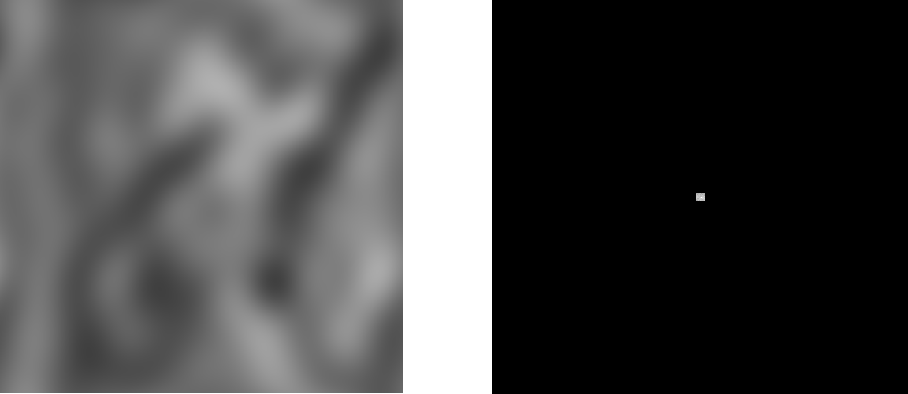
\includegraphics[width=0.6\textwidth]{fft_noise_10}
		\caption{Number of low frequencies: $10^2$}
		\label{fig:fft_10}
	\end{center}
	
\end{figure}

\begin{figure}[H]
	\begin{center}
		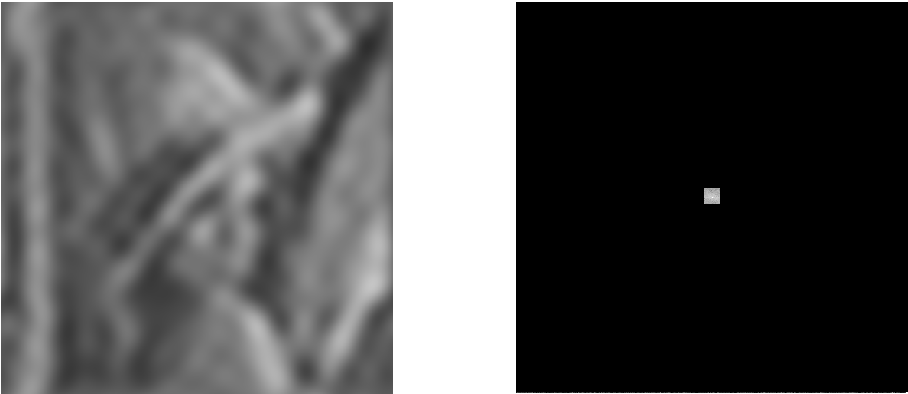
\includegraphics[width=0.6\textwidth]{fft_noise_20}
		\caption{Number of low frequencies: $20^2$}
		\label{fig:fft_20}
	\end{center}
\end{figure}

\begin{figure}[H]
	\begin{center}
		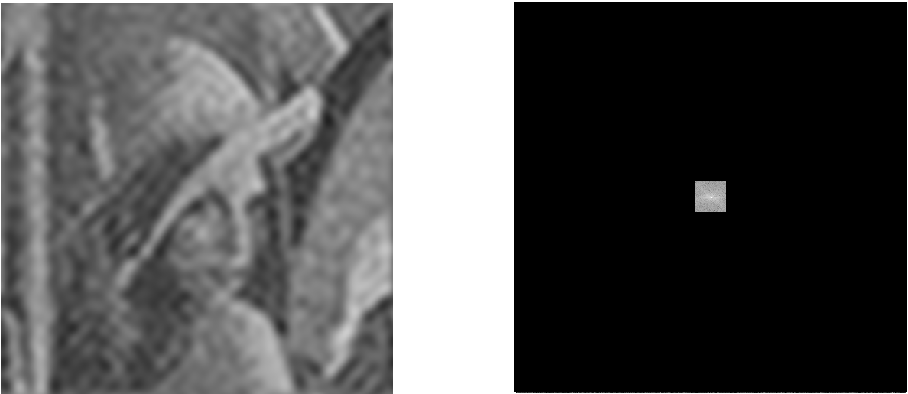
\includegraphics[width=0.6\textwidth]{fft_noise_40}
		\caption{Number of low frequencies: $40^2$}
		\label{fig:fft_40}
	\end{center}
\end{figure}

\begin{figure}[H]
	\begin{center}
		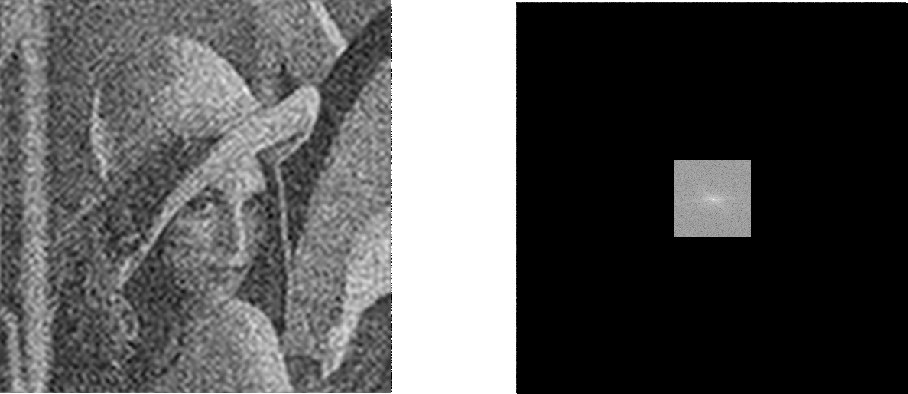
\includegraphics[width=0.6\textwidth]{fft_noise_100}
		\caption{Number of low frequencies: $100^2$}
		\label{fig:fft_100}
	\end{center}
\end{figure}

\begin{figure}[H]
	\begin{center}
		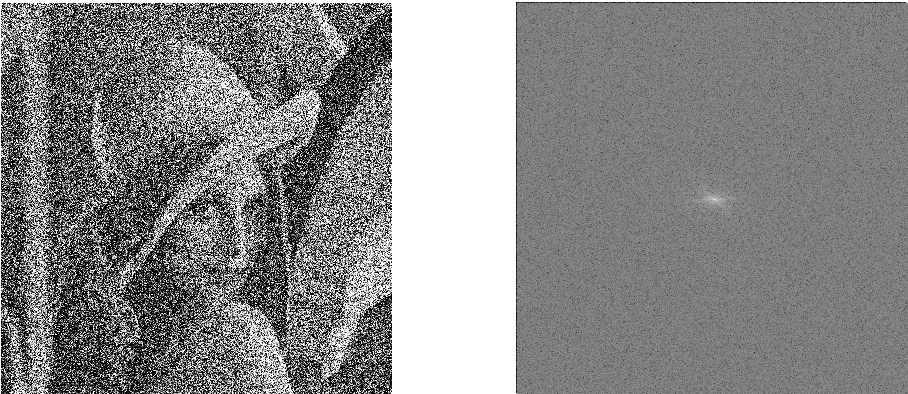
\includegraphics[width=0.6\textwidth]{fft_noise_full}
		\caption{Original Image}
		\label{fig:fft_full}
	\end{center}
\end{figure}
    

%% Problem 3
\item The problem is to implement a ROF model for total variation denoising. First, energy function and gradient function of it are derived. The original noisy image is shown on Figure~\ref{fig:noisy_img}. In order to perform iterations, parameters including epsilon,learning rate (lr), lambda and initial values of u are initialized. Then I iteratively perform gradient descent algorithm on the estimated image u. The energy loss keeps decreasing and converges after about 80 iterations (Figure:~\ref{fig:graph}). Central difference is applied to calculate gradient of the image. After it converges, u is optimized shown on Figure:~\ref{fig:denoised}.

\begin{figure}[h]
\begin{center}
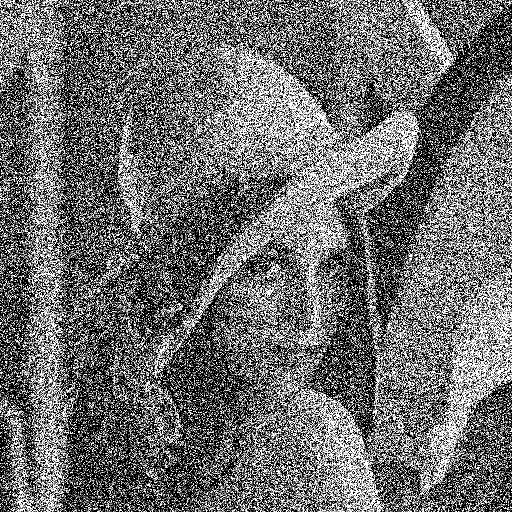
\includegraphics[width=0.4\textwidth]{../ProblemSet/lenaNoise.png}
\caption{Original Noisy Image}
\label{fig:noisy_img}
\end{center}
\begin{center}
	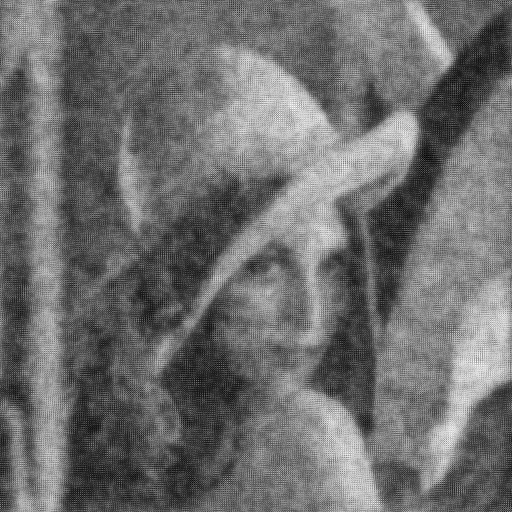
\includegraphics[width=0.4\textwidth]{../ProblemSet/code/denoised_img.png}
	\caption{Denoised Image}
	\label{fig:denoised}
\end{center}
\begin{center}
	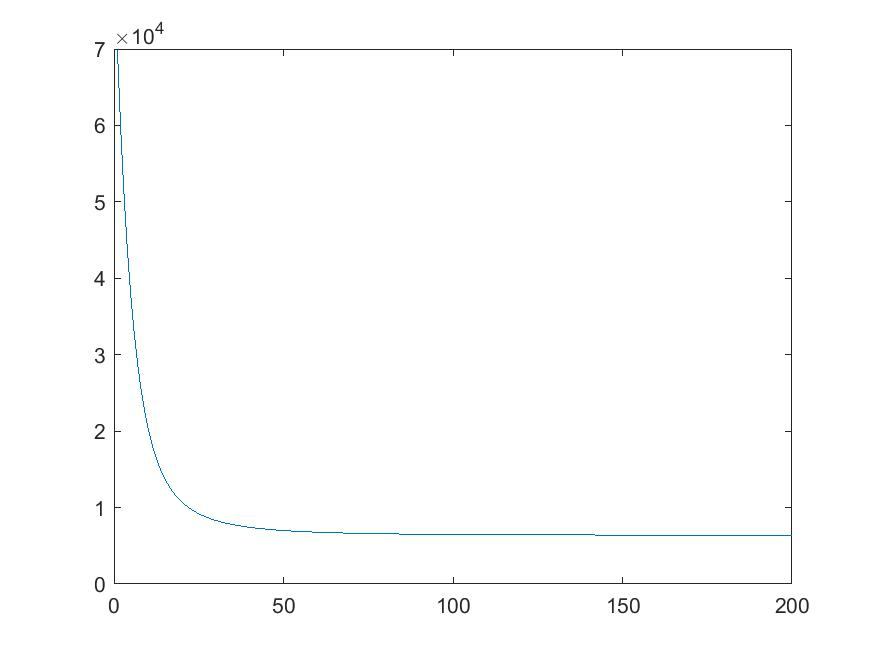
\includegraphics[width=0.4\textwidth]{../ProblemSet/code/gd_graph.jpg}
	\caption{Graph of Decreasing Loss}
	\label{fig:graph}
\end{center}
\end{figure}


\end{enumerate}

\end{document}
